% -*- program: xelatex -*-

\documentclass[12pt, t]{beamer}
%%% ------------------------------------------------------------------------
% packages
\usepackage{tikz}
\usetikzlibrary{shapes.geometric, arrows, positioning, shapes, backgrounds}
\usepackage{graphicx}
\usepackage{lmodern}
\usepackage{adjustbox}
% conditional (for figures)
\usepackage{etoolbox}

\usepackage{fontspec}
\usepackage{fontawesome}

\usepackage{subcaption} % side-by-side figures
\usepackage{hyperref}

\newtoggle{dark}

%%% ------------------------------------------------------------------------
% Theming (dark or white)
\usetheme{default}
\useoutertheme[subsection=false]{miniframes}

% move navigation to footer
\setbeamertemplate{headline}{}
\makeatletter
\setbeamertemplate{footline}
  {%
  \begin{beamercolorbox}{section in head/foot}
    \vskip2pt\insertnavigation{\paperwidth}\vskip5pt
  \end{beamercolorbox}%
  }
\makeatother


% no navigation bar
\beamertemplatenavigationsymbolsempty

% switch!
\toggletrue{dark}
% \togglefalse{dark}

\iftoggle{dark}{%
	% some colors
	\definecolor{foreground}{RGB}{255,255,255}
	\definecolor{background}{RGB}{24,24,24}
	\definecolor{title}{RGB}{127,185,220}
	\definecolor{gray}{RGB}{116,116,116}
	\definecolor{hilight}{RGB}{250, 108, 0}
	\setbeamercolor{section in head/foot}{fg = title}
	% set colors for titles, etc.
	\setbeamercolor{titlelike}{fg=title}
	\setbeamercolor{subtitle}{fg=title}
	\setbeamercolor{institute}{fg=gray}
	\setbeamercolor{normal text}{fg=foreground,bg=background}
	% % set colors for itemize
	\setbeamercolor{item}{fg=title} % color of bullets
	\setbeamercolor{subitem}{fg=gray}
	\setbeamercolor{itemize/enumerate subbody}{fg=gray}
}{
	% some colors
	\definecolor{foreground}{RGB}{0, 0, 0}
	\definecolor{background}{RGB}{255,255,255}
	\definecolor{title}{RGB}{107,174,214}
	\definecolor{gray}{RGB}{116,116,116}
	\definecolor{hilight}{RGB}{228, 97, 0}
	\setbeamercolor{section in head/foot}{fg = title}
	% set colors
	\setbeamercolor{titlelike}{fg=title}
	\setbeamercolor{subtitle}{fg=title}
	\setbeamercolor{institute}{fg=gray}
	\setbeamercolor{normal text}{fg=foreground,bg=background}
	% set colors for itemize
	\setbeamercolor{item}{fg=foreground} % color of bullets
	\setbeamercolor{subitem}{fg=gray}
	\setbeamercolor{itemize/enumerate subbody}{fg=gray}
}


%%% ------------------------------------------------------------------------
% Meta
\title{My work @QuantLandscapeEcology}   
\author{Eduard Szöcs} 
\institute{Institute for Environmental Sciences, University of Koblenz-Landau}
\date{Landau, 01.03.2016}



%%% ------------------------------------------------------------------------
\begin{document}
\begin{frame}
\titlepage
\end{frame}


%%% -------------------------------
\section{General} 
\subsection{}
\begin{frame}
\frametitle{My field of research is somewhere between...}
\center

\includegraphics[width =.8\textwidth]{fig/wordcloud_abstracts_firstauthor.png} \\	
\mbox{... Eco(toxico-)logy, Statistics, Data analyses and Programming}
\end{frame}


\begin{frame}
\frametitle{My philosophy: reproducible and open}
\vspace{1em}
\begin{description}
	\item[reproducible: ]{always!}
	\item[open: ]{as much as I  am allowed}
\end{description}
\vfill
Tools I am using and developing:\\[1em]
\begin{adjustbox}{max totalsize={1\textwidth}{\textheight},center}
\begin{tikzpicture}
	\definecolor{gray2}{RGB}{230,230,230}
	\tikzstyle{every node}=[font=\LARGE]
    \begin{scope}[fill opacity=0.5, text opacity=1]
		%R
		\filldraw[fill=gray2] (0cm,0cm) circle (1.5cm) node [inner sep=0pt] {
\includegraphics[width=2.5cm]{/home/edisz/Documents/Uni/Projects/PHD/MISC/AG_presentations/two/fig/R.png}};
		% PostgreSQL
   		\filldraw[fill=gray2] (2.7cm,0cm) circle (1.5cm) node [inner sep=0pt] {
\includegraphics[height=2.cm]{/home/edisz/Documents/Uni/Projects/PHD/MISC/AG_presentations/two/fig/postgresql.png}};
		% PostGIS
   		\filldraw[fill=gray2] (5.4cm,0cm) circle (1.5cm) node [inner sep=0pt] {
\includegraphics[height=2.cm]{/home/edisz/Documents/Uni/Projects/PHD/MISC/AG_presentations/two/fig/postgis.png}};
		% GRASS
		 \filldraw[fill=gray2] (8.1cm,0cm) circle (1.5cm) node [inner sep=0pt] {
\includegraphics[height=2.cm]{/home/edisz/Documents/Uni/Projects/PHD/MISC/AG_presentations/two/fig/grass.png}};
		% LATEX
		 \filldraw[fill=gray2] (10.8cm,0cm) circle (1.5cm) node [inner sep=0pt] {
\includegraphics[width=2.cm]{/home/edisz/Documents/Uni/Projects/PHD/MISC/AG_presentations/two/fig/latex.png}};
		% github
		\filldraw[fill=gray2] (13.5cm,0cm) circle (1.5cm) node [inner sep=0pt] {
\includegraphics[width=3cm]{/home/edisz/Documents/Uni/Projects/PHD/MISC/AG_presentations/two/fig/github.png}};
    \end{scope}
\end{tikzpicture}
\end{adjustbox}
\end{frame}




\section{Monitoring data}
\subsection{}
\begin{frame}
\frametitle{I - Compilation of chemical monitoring data}
\begin{adjustbox}{max totalsize={.9\textwidth}{.8\textheight},center}
	\begin{tikzpicture}
		\definecolor{gray2}{RGB}{230,230,230}
		\definecolor{gray3}{RGB}{157,177, 204}
		\definecolor{green}{RGB}{109,198,112}
		\definecolor{blue}{RGB}{64,130,237}
		\tikzstyle{every node}=[font=\LARGE]
		\begin{scope}[fill opacity=0.5, text opacity=1]
			\filldraw[fill=blue] (2.12cm:12cm) circle (2.5cm) node[text width=4cm,align=center]{Chemical \\ properties};
			\filldraw[fill=green] (3.1cm:10.5cm) circle (2.5cm) node[text width=4cm,align=center]{Legislation};
			\filldraw[fill=title] (0cm,0cm) circle (4cm) node[text width=4cm,align=center]{Biological\\monitoring};
			\filldraw[fill=hilight] (0cm:6cm) circle (4cm) node[text width=4cm,align=center]{Spatial data};
			\filldraw[fill=gray3] (2.12cm:6cm) circle (4cm) node[text width=4cm,align=center]{Chemical \\ monitoring};
			\node[inner sep=0pt] (logo) at (14,-4) {
\includegraphics[width=0.7\textwidth]{fig/bfg_uba.png}};
		\end{scope}
	\end{tikzpicture}
\end{adjustbox}
\end{frame}

\begin{frame}
\frametitle{I - Data overview}
\begin{table}[htbp]
\scriptsize
\begin{tabular}{lllrrr}
type & start* & end & no. sites & no. samples & no. variables \\ \hline
pesticides & 2005-01-02 & 2015-03-25 & 3112 & 46295 & 491 \\ 
biological & 2005-01-11 & 2013-11-29 & 14211 & 27392 & 2824 \\ \hline
\end{tabular}
\end{table}

\begin{figure}
\centering
\begin{subfigure}{.5\textwidth}
  \centering
  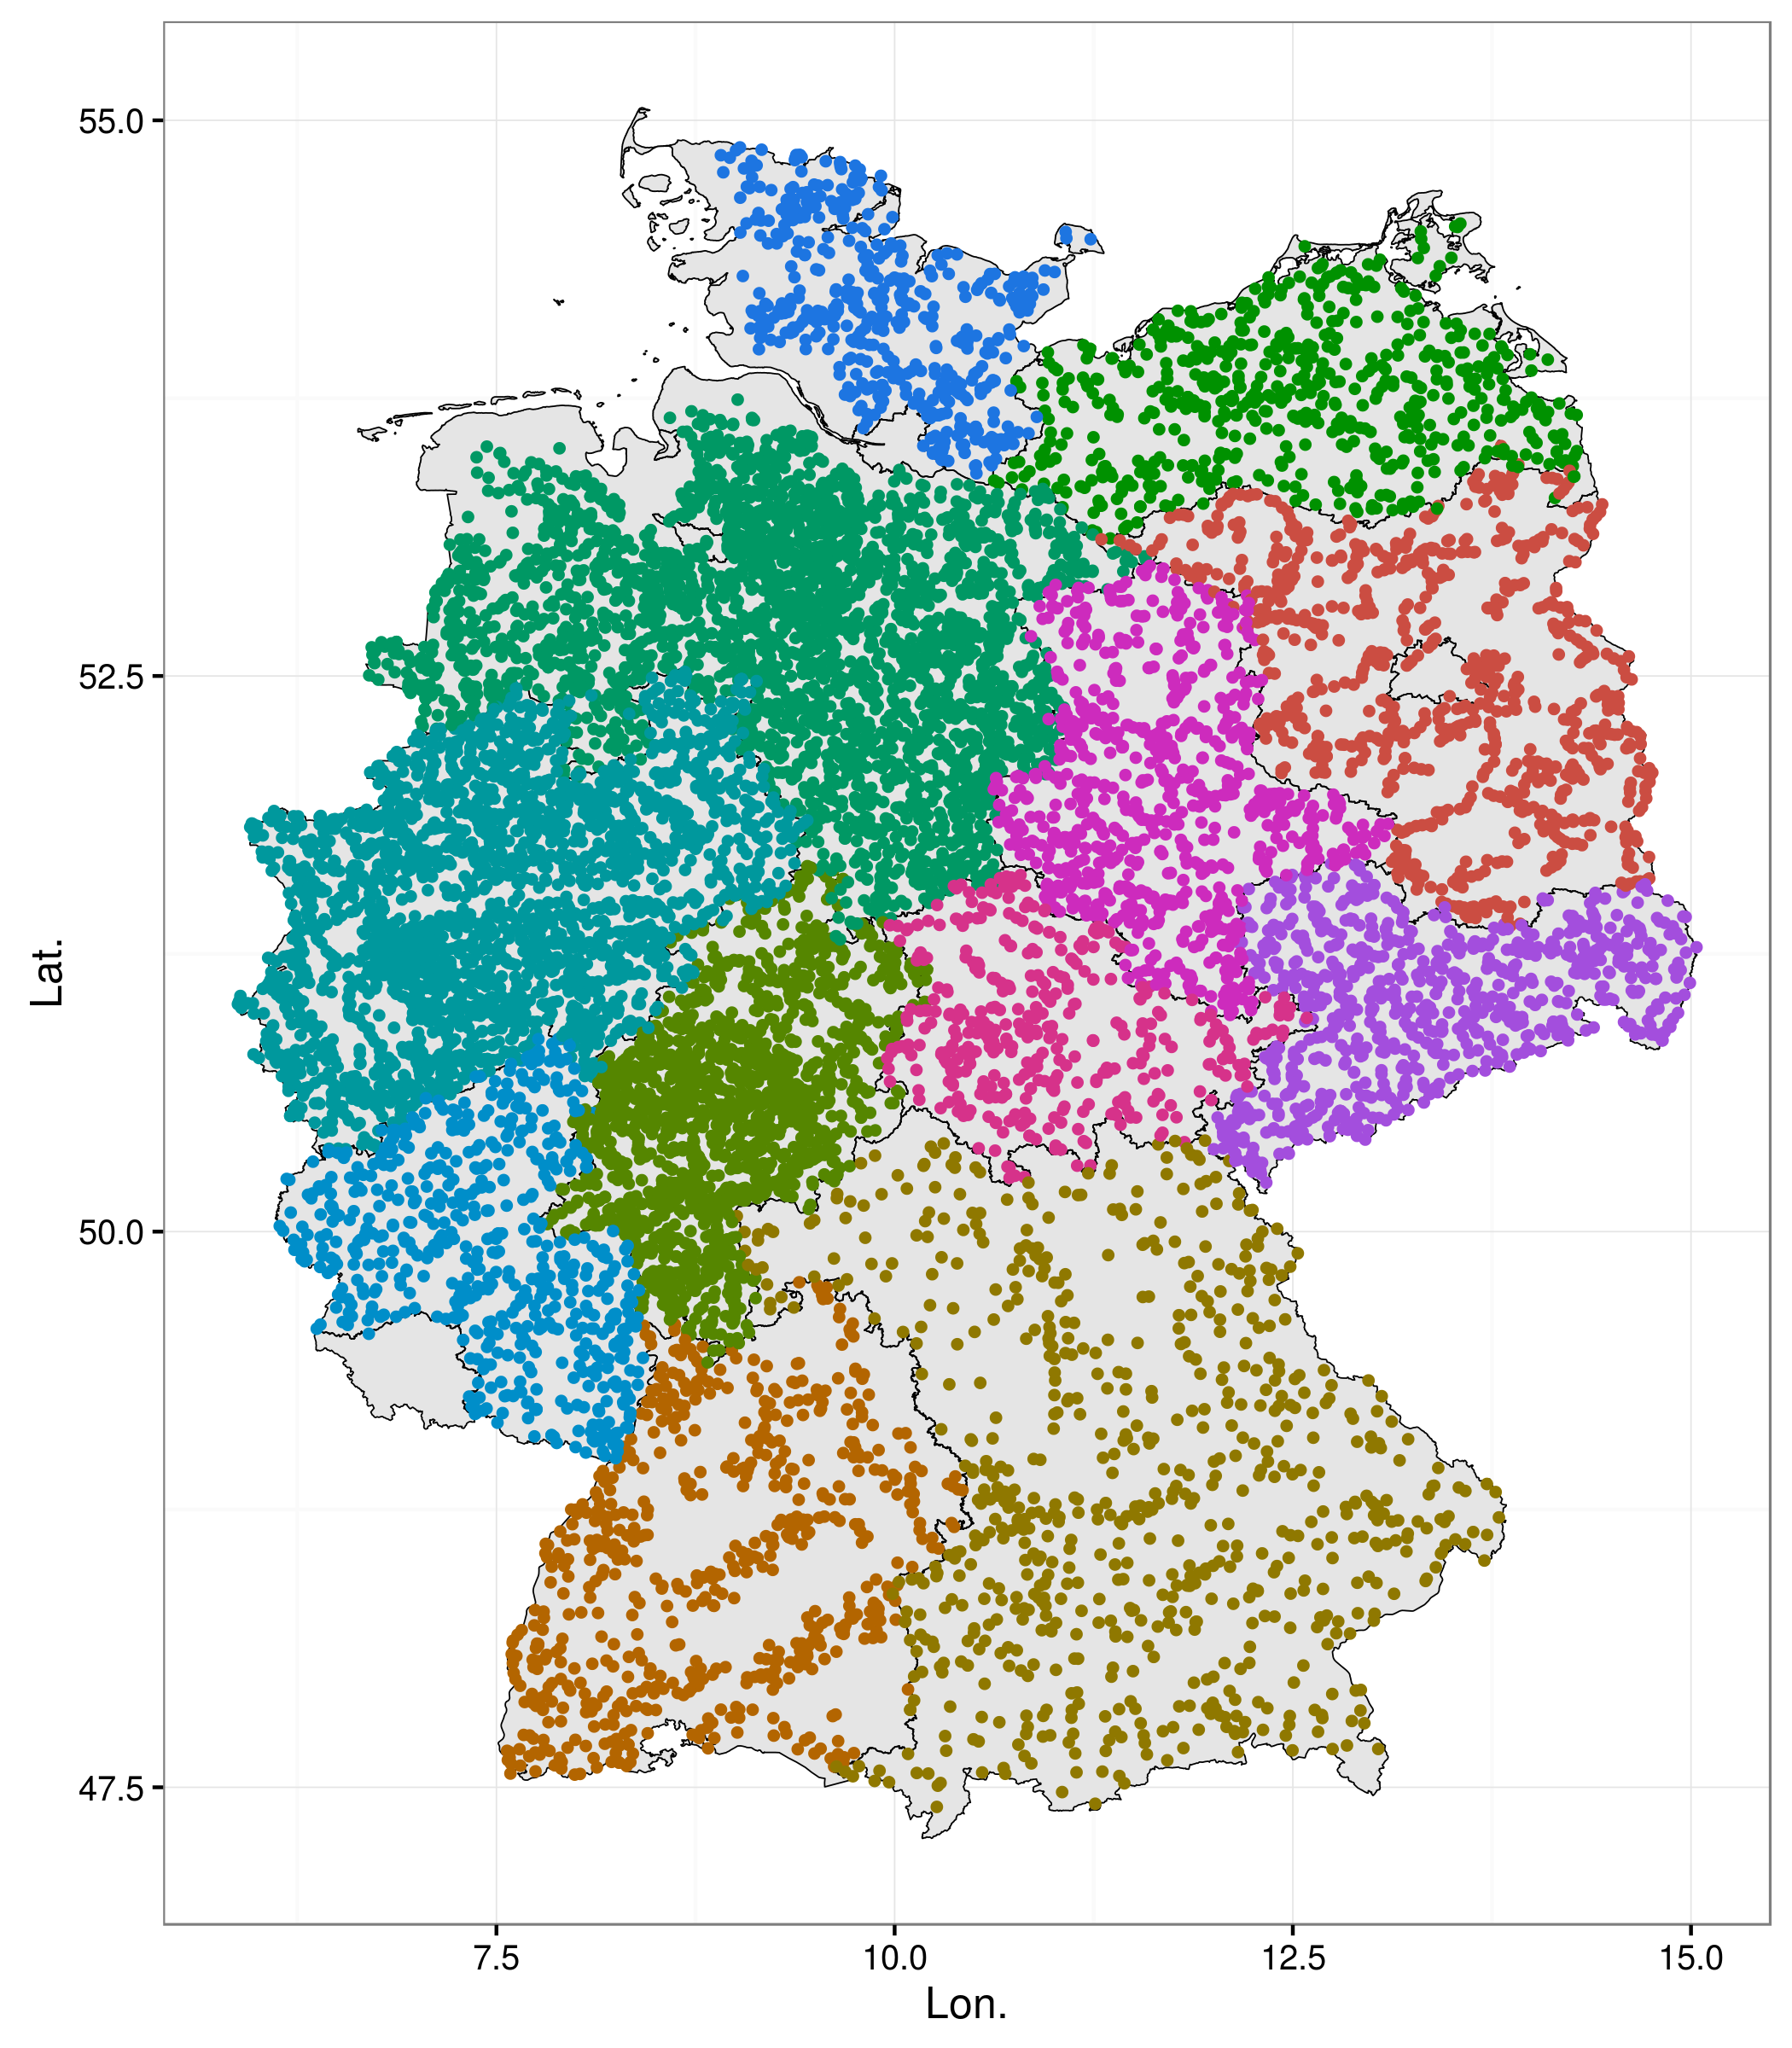
\includegraphics[width=\linewidth]{fig/mzb_map.png}
\end{subfigure}%
\begin{subfigure}{.5\textwidth}
  \centering
  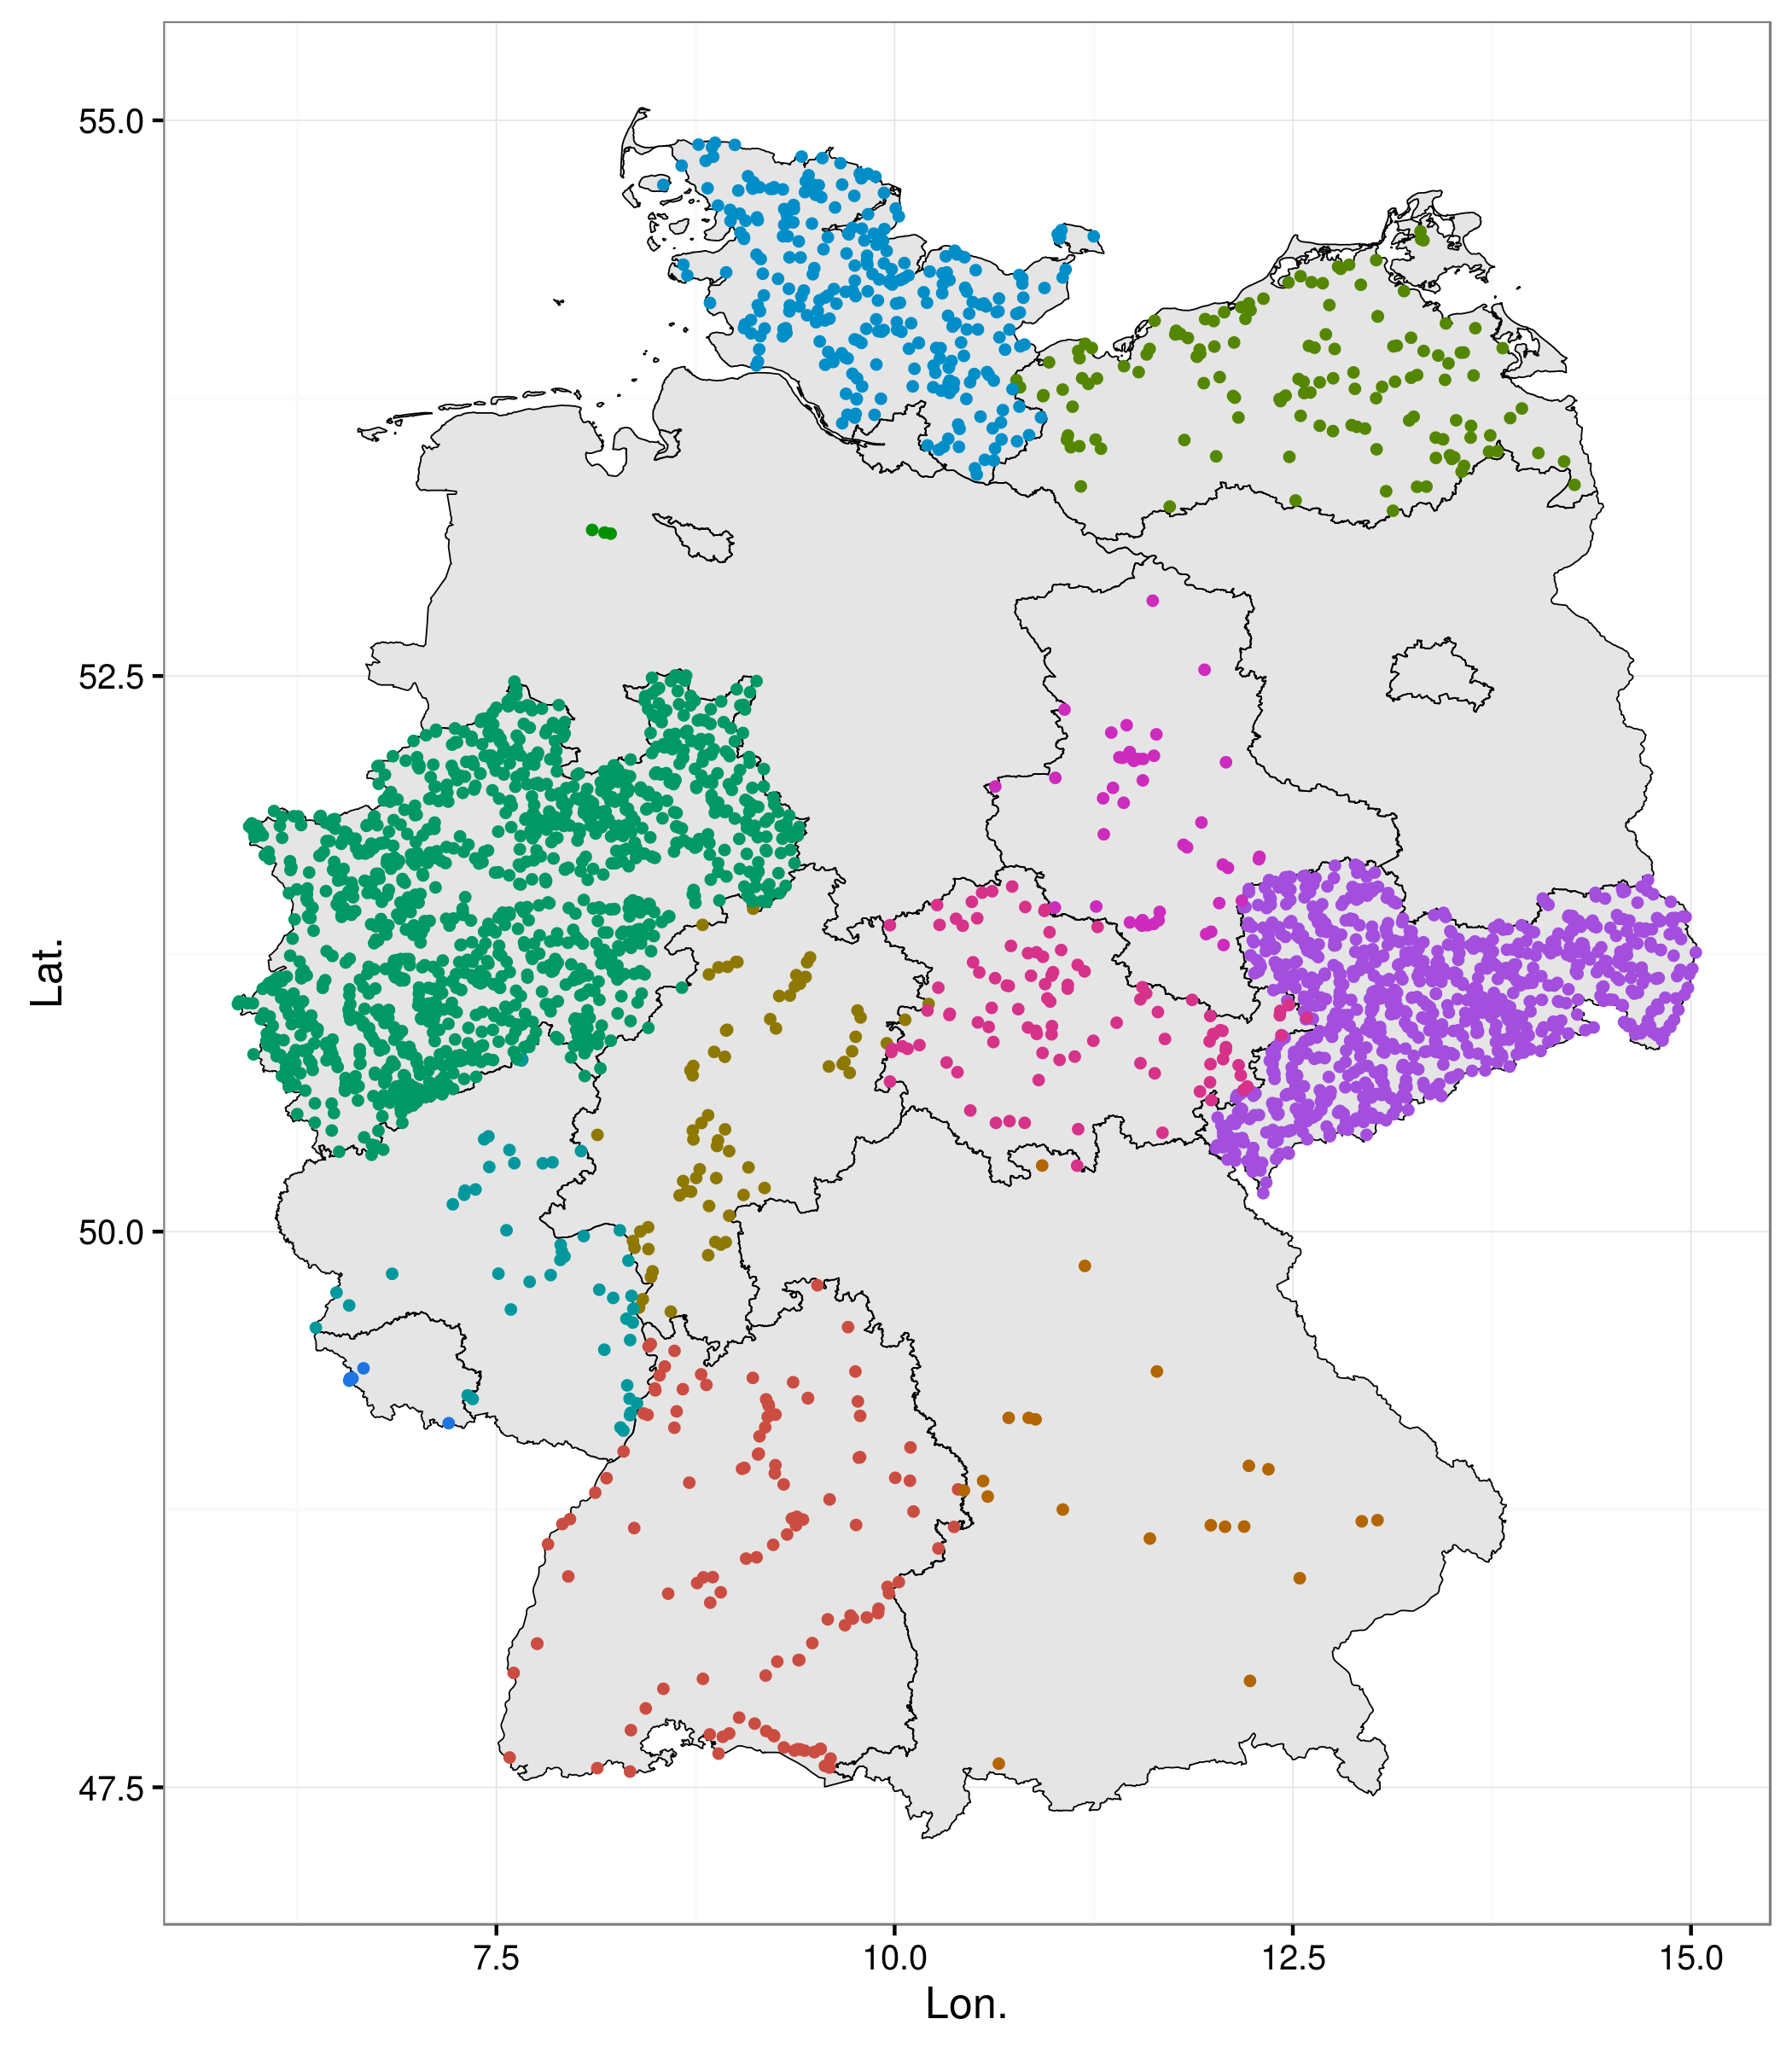
\includegraphics[width=\linewidth]{fig/phch_map.png}
\end{subfigure}
\end{figure}
\end{frame}

\begin{frame}
\frametitle{I - What do we know about small water bodies?}
\begin{figure}
\centering
\begin{subfigure}{.5\textwidth}
  \centering
    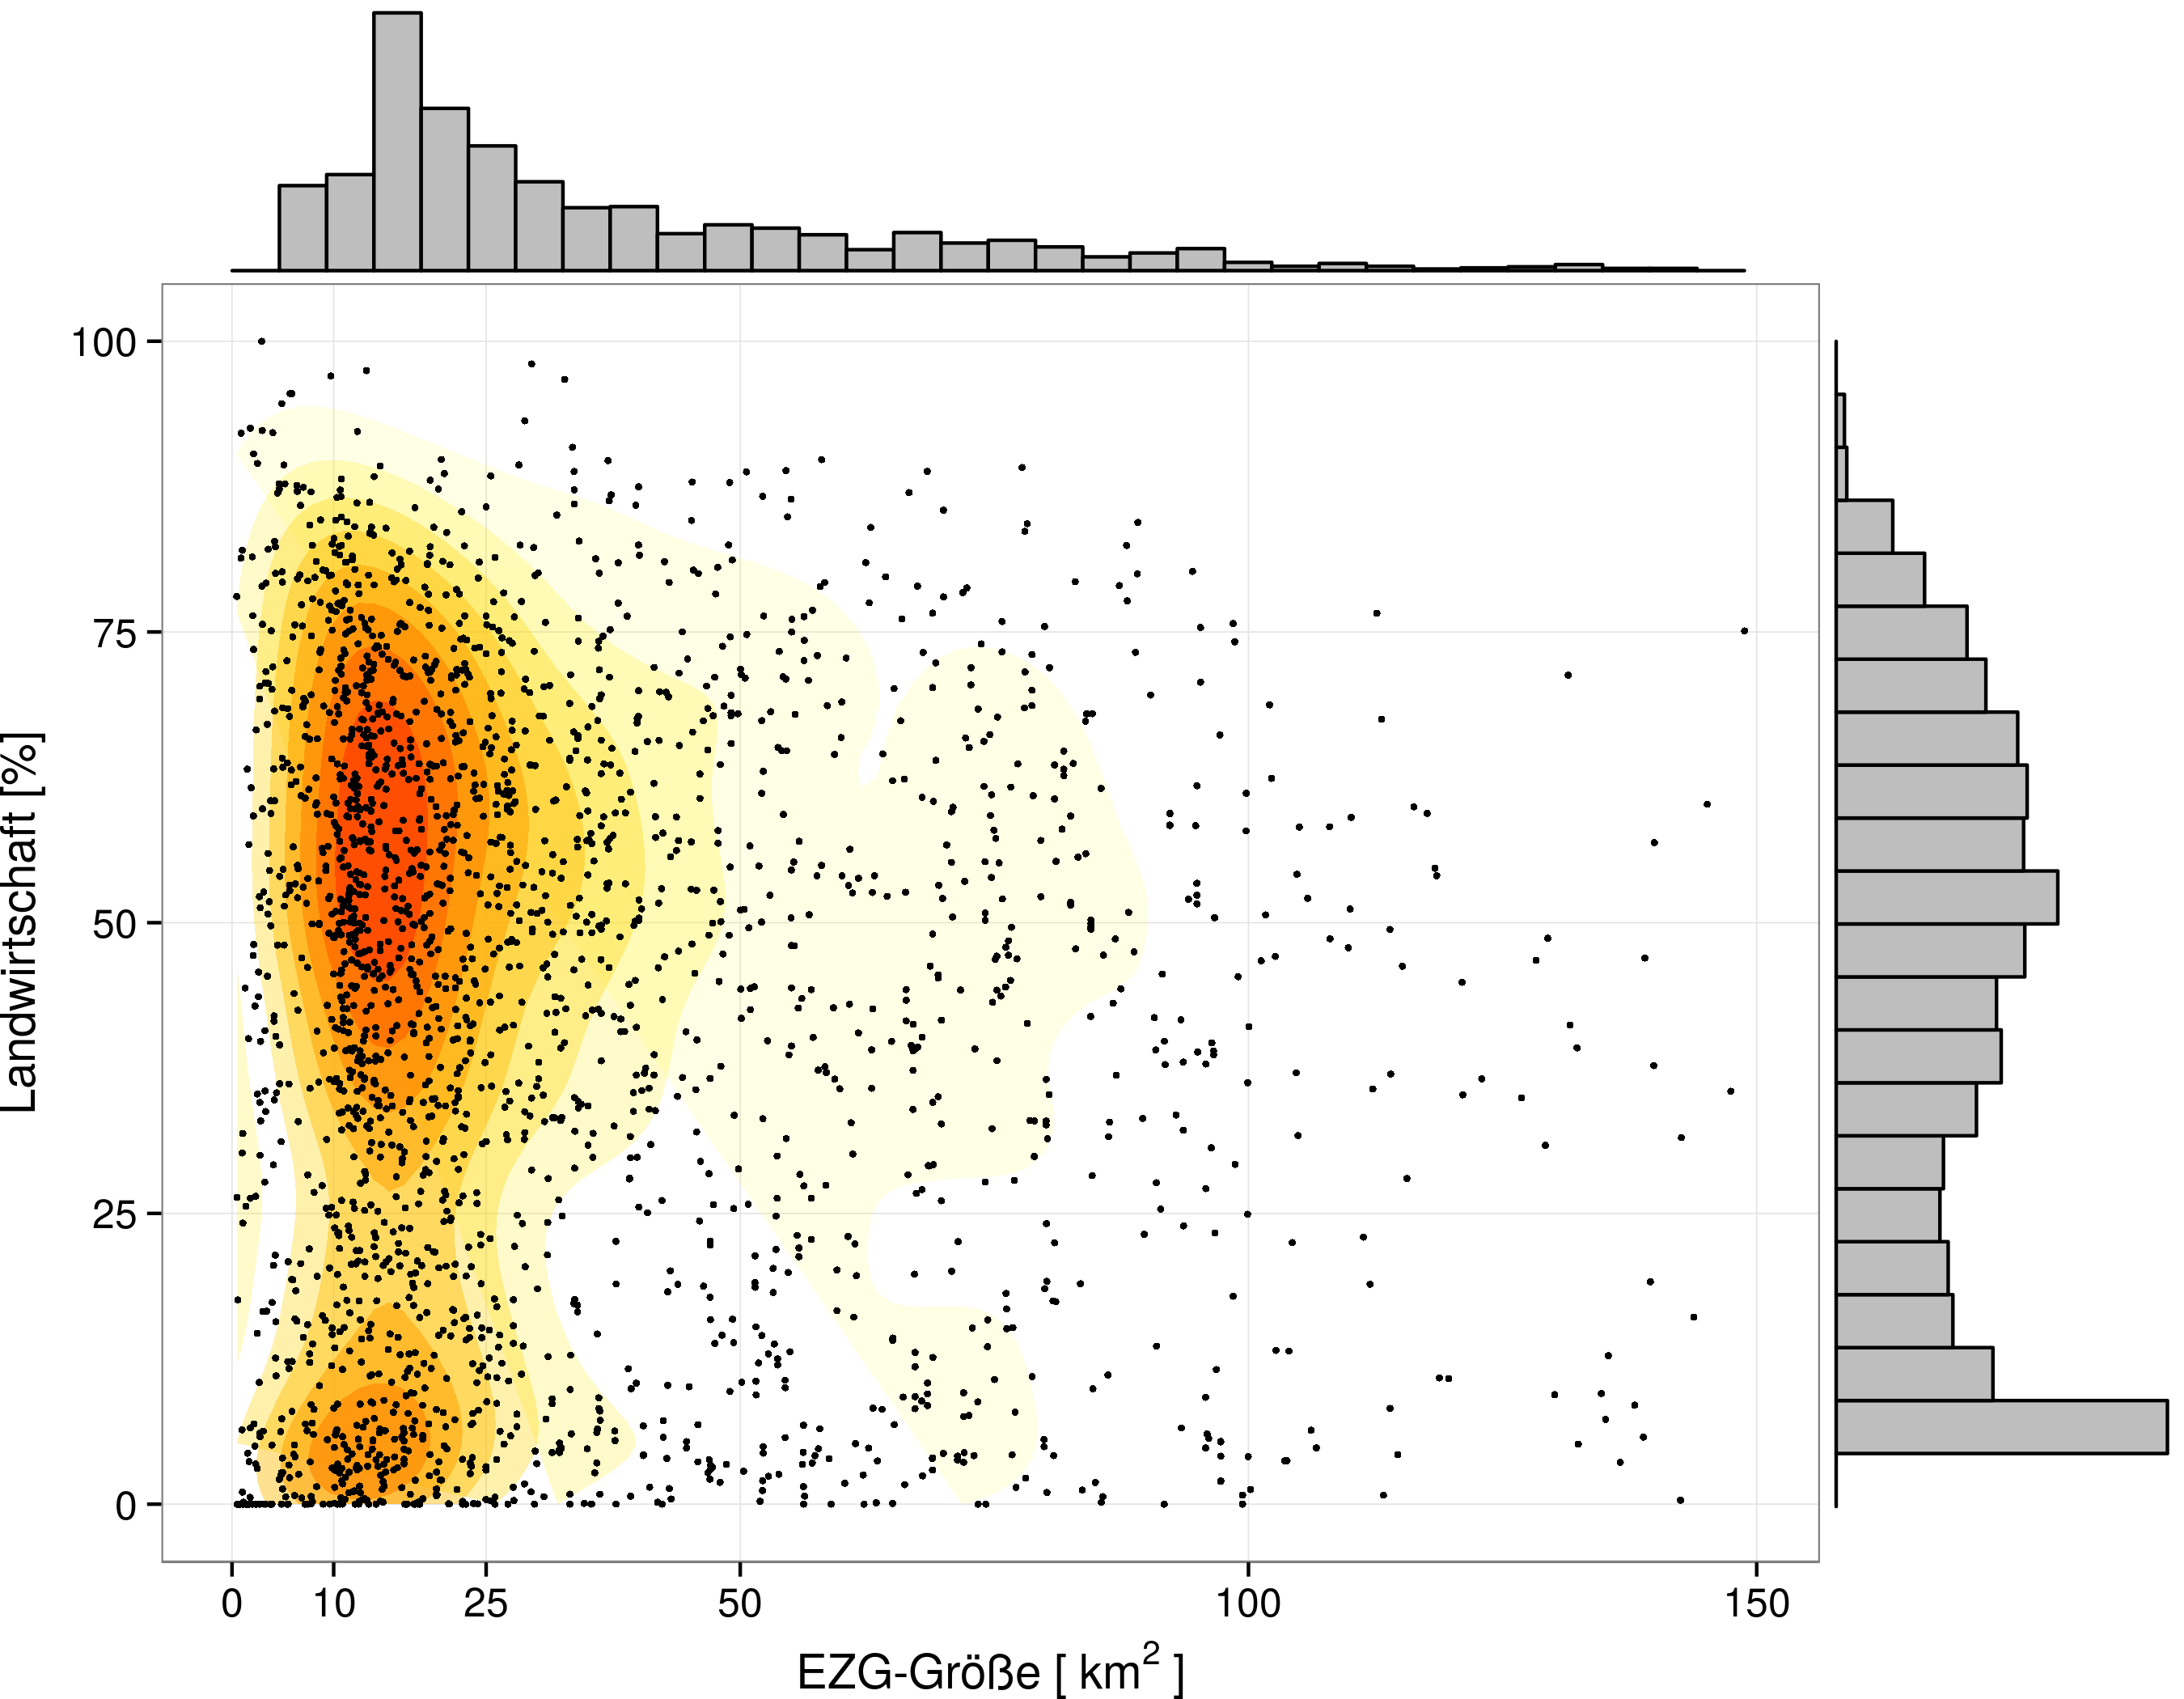
\includegraphics[width=\linewidth]{fig/ezg_lu.png}

\end{subfigure}%
\pause
\begin{subfigure}{.5\textwidth}
  \centering
  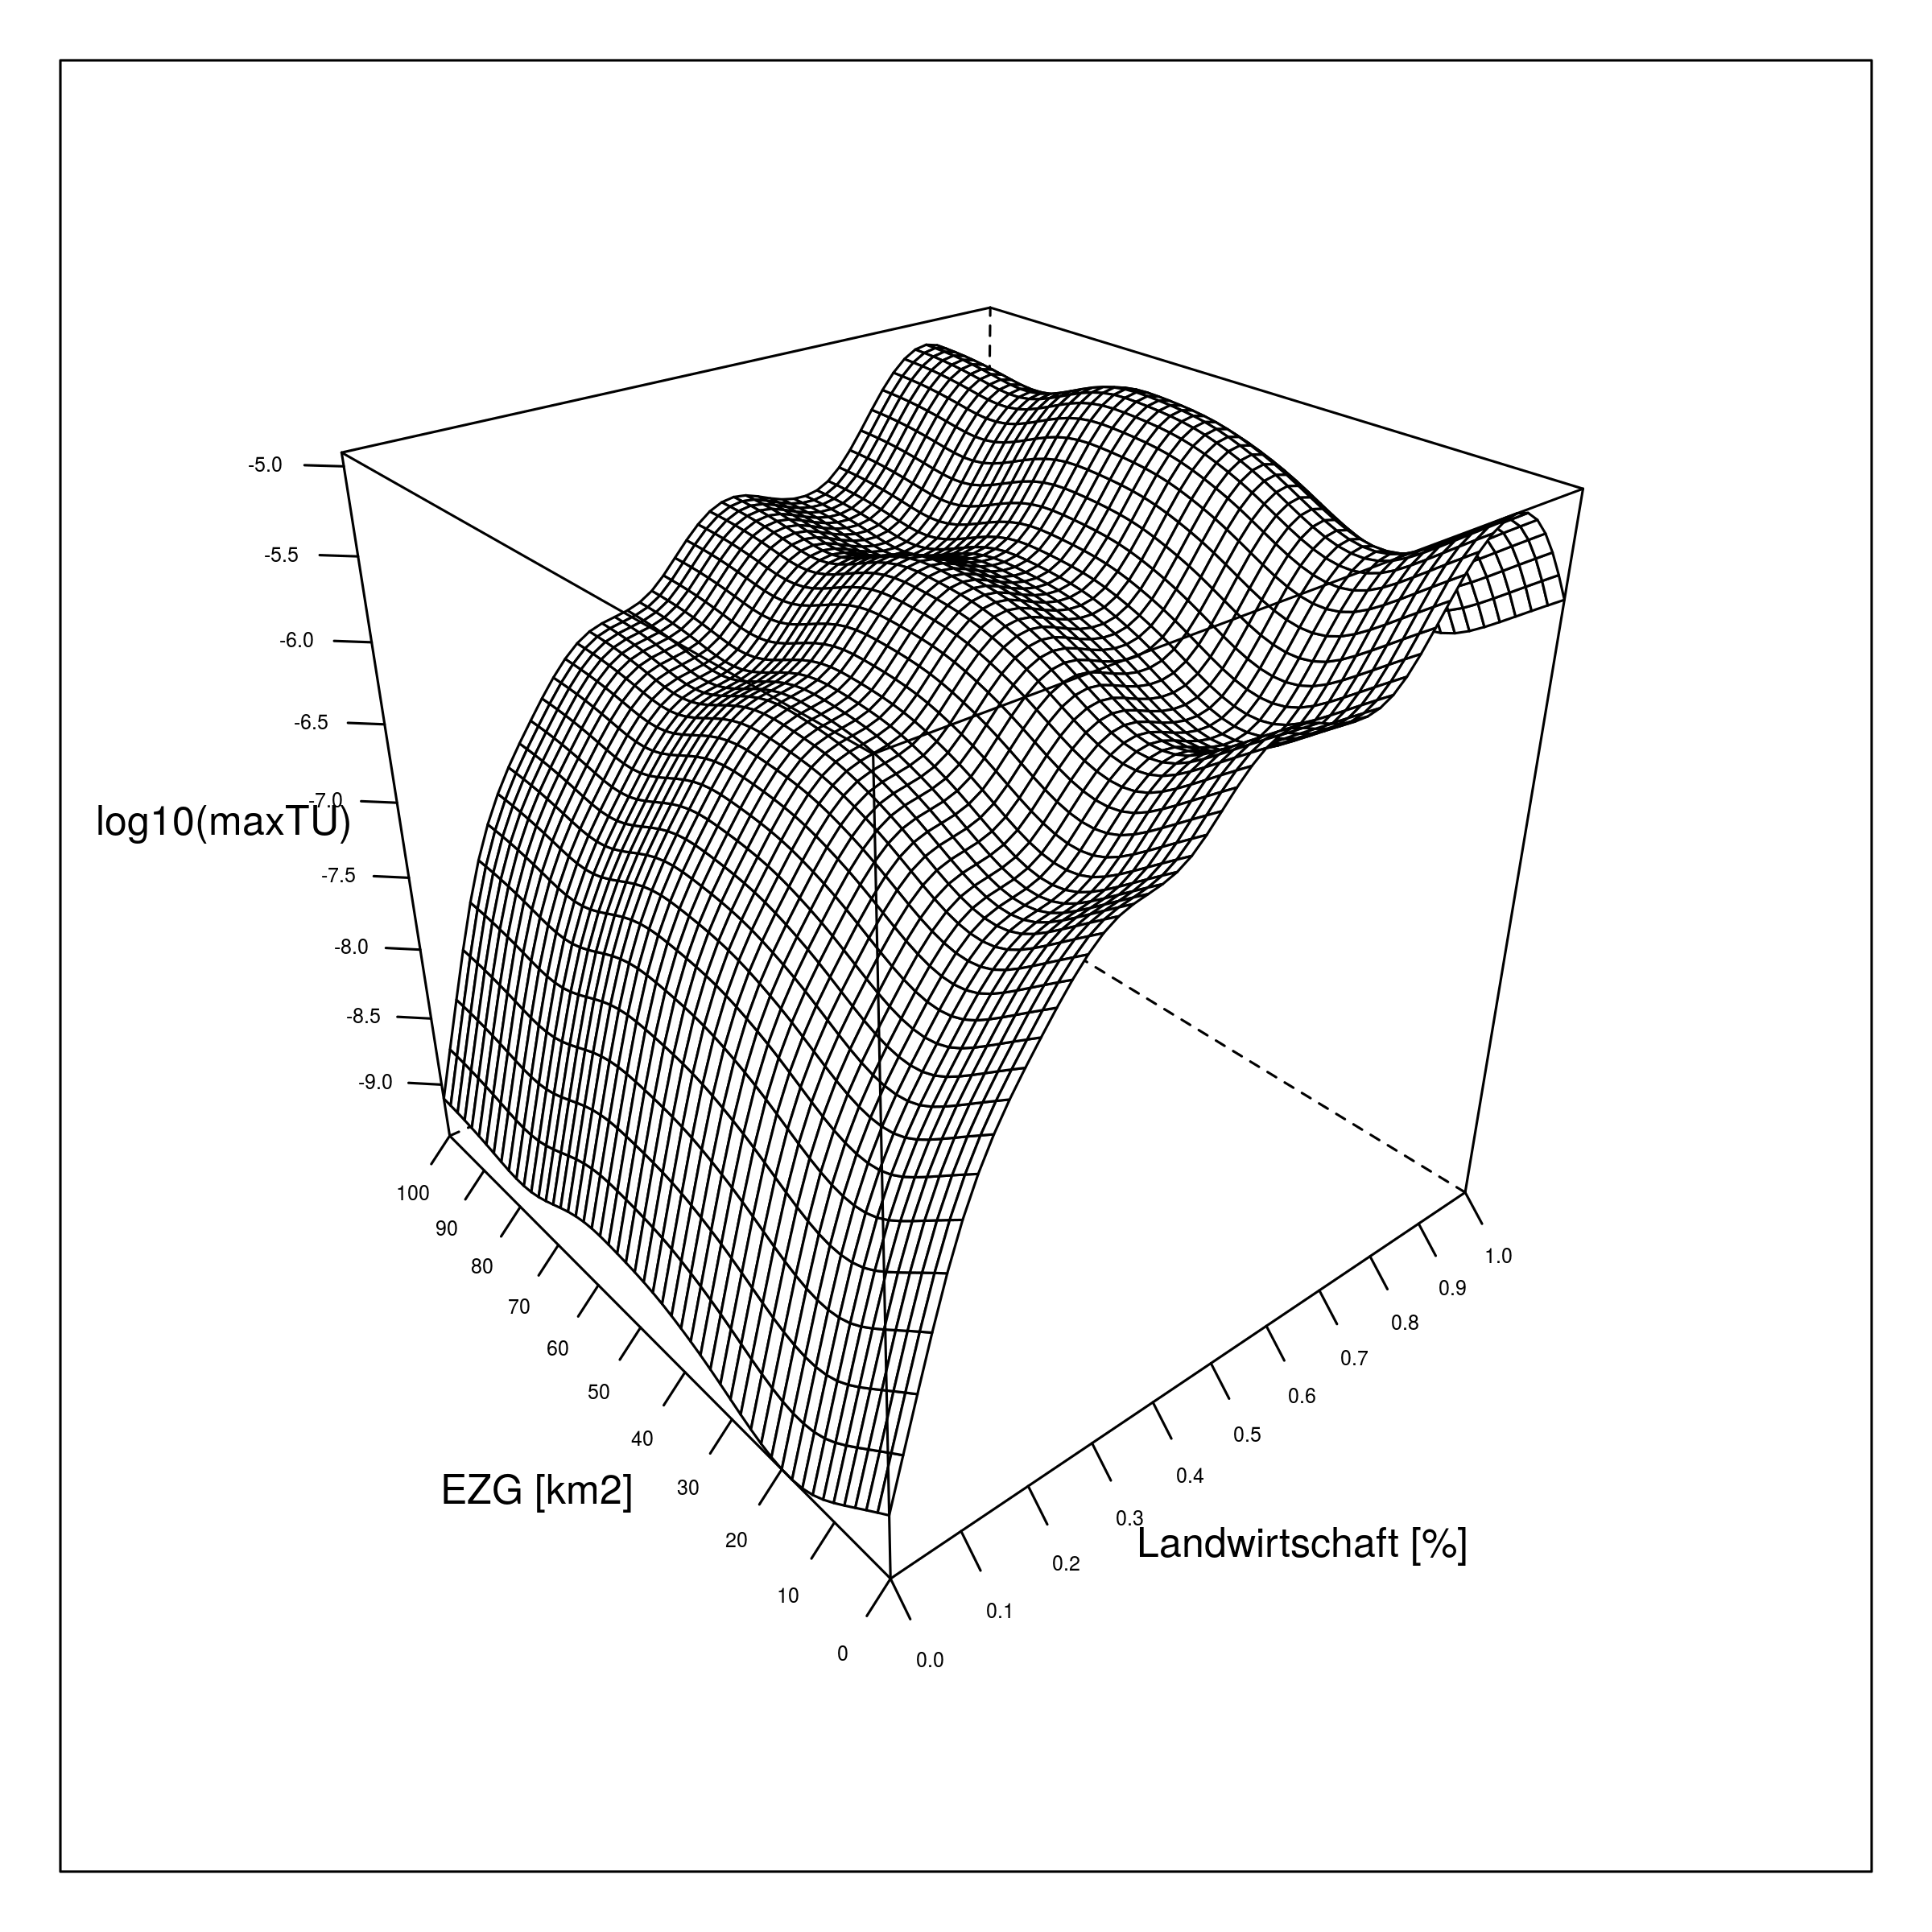
\includegraphics[width=\linewidth]{fig/lu_ezg_agri_cens.png}
\end{subfigure}
\end{figure}
Other questions / analyses are in the pipeline...
\end{frame}


\section{Programming}
\subsection{}
\begin{frame}
\frametitle{II - Develop tools to handle such data}
\vspace{1em}
Mainly R-packages:

\begin{description}
	\item[taxize: ] Cleaning and handling \textcolor{hilight}{taxonomic} data.
	\item[webchem: ] Search \textcolor{hilight}{chemical} information.
	\item[other: ] vegan-package, resolving ambiguous taxa, ...
\end{description}
\vfill
\colorbox{white}{
\includegraphics[width =.3\textwidth]{fig/ropensci.png}}
\end{frame}



\section{Other stuff}
\subsection{}
\begin{frame}
\frametitle{III - Other stuff I am working on}
\vspace{1em}
\begin{description}
\setlength\itemsep{1em}
\item[Field study:  ]{Organization, communication, field work, ...	}
\item[Statistics: ] {
	\begin{itemize}
		\item Methods to analyse mesocosm data
		\item Methods to model non-linear non-normal censored data
		\item Help out my nice colleagues
	\end{itemize}
}
\item[Freelance: ] {
	\begin{itemize}
		\item in my (rare) free time...
		\item R Courses
		\item Data sourcing, cleaning \& analysis
	\end{itemize}
}
\end{description}
\end{frame}



\begin{frame}
\frametitle{}
\vspace{1em}
\begin{centering}
\Large \textcolor{title}{Data in Eco(toxico)logy} \\[1em]
Eduard Szöcs \\[0.3em]
\tiny \textcolor{gray}{Institute for Environmental Sciences, University of Koblenz-Landau} \\[5em]
\end{centering}
\normalsize
\textcolor{hilight}{\faLaptop}~~~\href{http://edild.github.io/}{http://edild.github.io/ }\\[.5em]
\textcolor{hilight}{\faTwitter}~~~\href{http://twitter.com/EduardSzoecs}{@EduardSzoecs} 	\\[0.5em]
\textcolor{hilight}{\faGift}~~~\href{https://github.com/edild/talk_work}{https://github.com/EDiLD/talk\_work}\\[0.5em]
\textcolor{hilight}{\faEnvelope}~~~\href{mailto:szoecs@uni-landau.de}{szoecs@uni-landau.de} \\[.5em]
\hfill 
\includegraphics[width =.3\textwidth]{fig/Cc-by-nc_euro_icon.png} 
\end{frame}


\end{document}